\section{Chatbot performance}
The nature of chatbot development is one of predicting what a user will say; this is already a hard job for any large software development effort, making it incredibly difficult for a single person team.
Testing on our own account, using phrasings we knew the chatbot would recognise, was very different from deploying it in the wild, and experiencing all the different ways participants in the study tried to express the same concepts. \\
Observing how the users were interacting with the chatbot made it clear that our design choice of minimising false negatives by using the @sys.any entity to capture food wasn't particularly successful. Users would often try to interact with the chatbot for non functional conversation, such as greeting it, thanking it about one of its encouragements to keep logging food, complaining about a mistake or simply acknowledging a previous message. In those cases, if the intent-triggered conversation had already been terminated, the new message would be incorrectly identified as food, without a quantity, and a clarification request message to specify the portion size would be fired. \\
\begin{figure}[h!]
  \centering
  \begin{subfigure}[b]{\linewidth}
    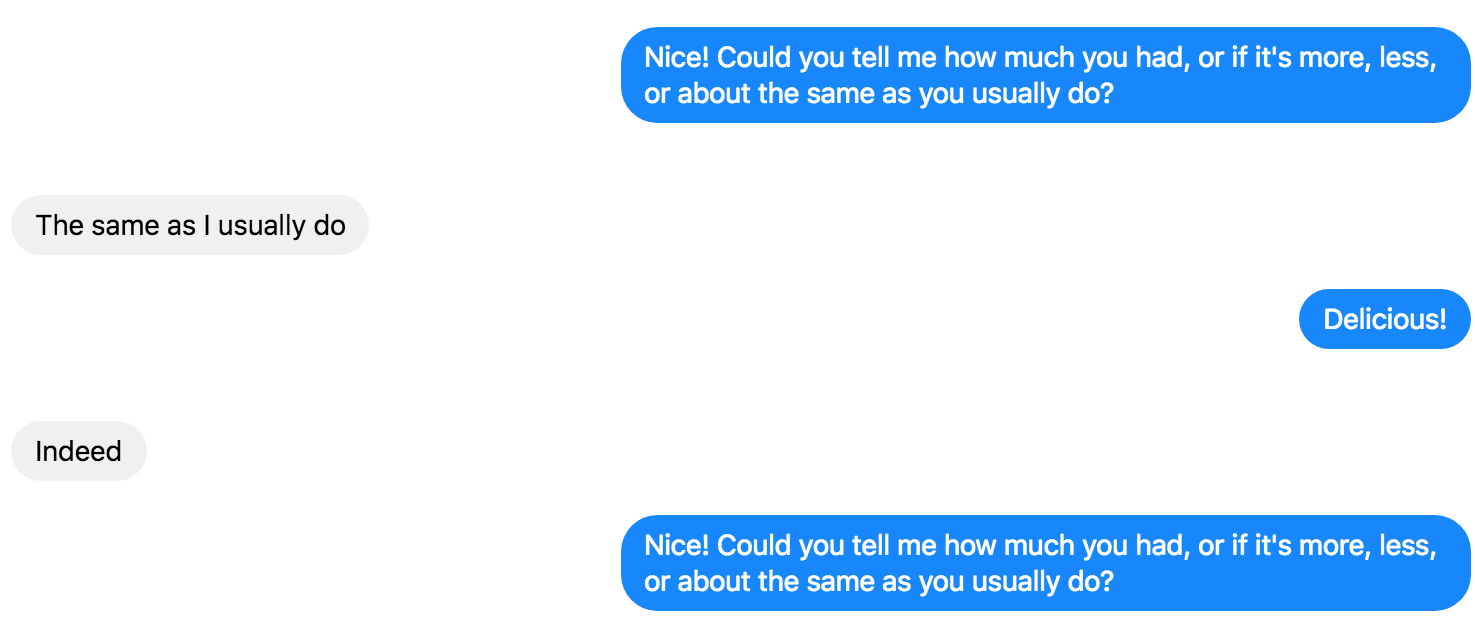
\includegraphics[width=\linewidth, height=6cm,keepaspectratio]{Nice.png}
     %\caption{Coffee.}
  \end{subfigure}
  \begin{subfigure}[b]{\linewidth}
    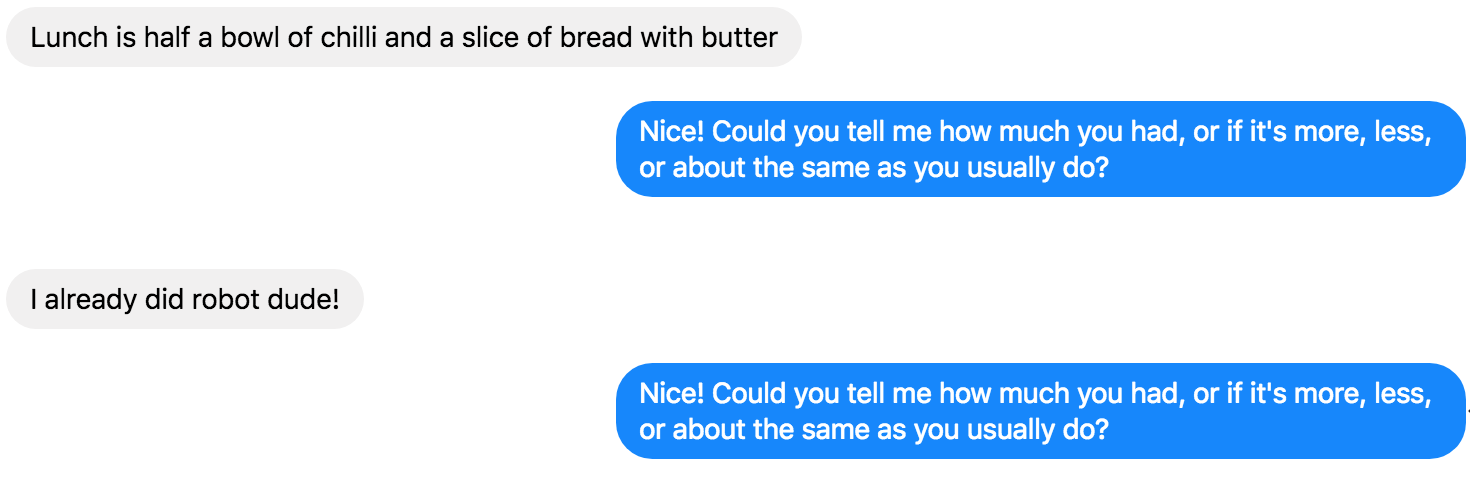
\includegraphics[width=\linewidth, height=6cm,keepaspectratio]{Nice2.png}
    %\caption{More coffee.}
  \end{subfigure}
\end{figure}
This also caused the intent recognition model to have several false positives, misidentifying stop words as food within a message that also contained valid food words. Fortunately, this kind of false positive turned out to be less relevant, because the user would already have to identify some portion sizes, so they wouldn't notice misidentification issues, and the recognised food was only stored in the database if matching with some record in the \textit{Nutritionix} API. But while the API did provide a safeguard against incorrect food identification, it also showed issues by misidentifying real food, either by catching only part of the word (cupcake was flagged as cake mix in one instance), or sometime inexplicably (Long island ice teas were stored in the database more than once, without the user having logged them). The ability to list several different food items within a single message, as well as users' habit of splitting up different elements of the same meal between different messages, also caused difficulties in matching quantity to food, with Dialogflow's models simply not being advanced enough to catch the many subtleties of word ordering. This was another cause for the size clarification message to be presented after a quantity had already been given.\\
The \textit{clarifai} API rarely conformed to our ideal parameter of a single identification over the 97\% confidence threshold; however, the among the top three choices, there was often a good candidate the user could choose to select. When confronted with no suitable choice, if the user tried to clarify what the food was, the chatbot appeared to recover gracefully, while actually logging the clarification as a new meal. \\
A considerable effect on how the chatbot performed with users was also due to operational issues. After obtaining consent to participate in the experiment, users were provided with a URL they could open through the Facebook Messenger app or in the browser. Before it became clear that individual users had to be added as testers through the Facebook developer console, the first users who were given a URL did not receive any reply to their messages until they were added. While it was explained to them that this was not an issue with the chatbot but a temporary account management problem, it might have contributed to the perception that the chatbot was buggy. In fact, even after testing initiated correctly, there were some uncaught bugs that users could easily spot, which betray the fact that they were conversing with an automaton. For many of the chatbots' interactions, responses were selected randomly from a predefined list; over time, the user would exhaust all variants for a response, and since these were selected randomly sometimes would have the exact same responses given to them in quick succession. Sometimes, the database would fail silently when accessing the user name, so a message would be sent to the user containing ``undefined'' rather than their name. Perhaps most grievously, an uncaught exception in the logic of ``worker.js'' caused the entire periodic reminder script to fail after having sent messages to the first user. Because the first user was our test account, we kept receiving reminders through the evaluation period, which caused us to believe everything was behaving correctly until the 6th day of the experiment. Since this was a very important feature we were interested in evaluating, we decided to push a fix in production, and to extend the trial by two more days to verify its effects. The fix was not perfect, causing the no log reminder to fire up for every user, even if they had just logged their food the night before. However, while this might have been annoying for these users, it proved highly effective, causing every single user to log at least a meal on the day and after, including those who had only tested it on the first day and given up after. The leafy greens reminder was also subjected to a similar bug, firing for every user just before the no log reminder. Unlike the latter, most users didn't seem to react to the suggestion, and while some registered the message, it's not clear whether users failed to modify their behaviours because the greens reminder encourages a more difficult change, or simply because they only noticed one of the remainders. The second explanation is not unlikely, given the fact that our testers seem to ignore larger body of text while messaging, like the introductory welcome message which explained the chatbot's capabilities, causing users who weren't given an explanation before the experiment to be unaware of some functionality.
%TODO randomization causes insensitive replies
\section{Evaluation results}
Responses to our survey confirmed that the chatbot is not ready for public release, and in its current incarnation provides little utility compared to app based food diaries; however, under some metrics the chatbot did provide a stronger performance, leaving open the possibility that after further work it might provide a suitable replacement. \\
While our study provides us with some interesting qualitative data, it should be noted that we cannot conduct hard generalisations on our results, because of the tiny sample size. Our participants come from the uniform demographic of university students because of issues with the logistics of recruitment; while this enables us to compare data without taking into account how demographics affect replies, it also means we lack external validity, and we cannot understand how other groups, especially vulnerable less tech-savy ages or people who have major dietary issues, will react. Further studies will be necessary to ascertain how usable the interface is for different demographics. \\





% discuss help and not reading in survey results for wanting more user features
Outside the survey During user evaluation, features were pointed out: clear record if incorrect food, add food on different date; users wanted more frequent reminders; didn't realise pictures capability, or lookback on food; reminders didn't work for the first 6 days, but when they were turned on 100\% of users went back in the same morning, and most sent a message after as well; bad interaction with follow ups

\section{Future improvements} 
% maybe goes in conclusion?

Features we want: recurring meals, GIFs, challenges
Vegans! Take goals and weights into account

Through the implementation, it became evident how little privacy a chatbot user can expect. No e2e encryption, data shared among chat provider, NLP tools, databases, cloud hosting and analytics

% cite MFP hack!!
% external validity much!! uniform population
